\documentclass[a4j,titlepage]{jsarticle}

\usepackage[dvipdfmx]{graphicx,xcolor}
\usepackage[top=20truemm,left=25truemm,right=25truemm]{geometry}
\usepackage{amsmath}
\usepackage{here}
\usepackage{comment}
\usepackage{url}
\usepackage{plistings}
\usepackage{tikz}
\usepackage[framemethod=tikz]{mdframed}

\renewcommand{\lstlistingname}{リスト}

\newcommand{\chuo}[1]{\multicolumn{1}{|c|}{#1}}
\newcommand{\inpt}[1]{\underline{#1}\,\setlength{\fboxsep}{1pt}\fbox{\small ↓}}
\newcommand{\bvec}[1]{\mbox{\boldmath $#1$}}

\lstdefinestyle{C}{
  language=C,
  basicstyle=\small\ttfamily,
  keywordstyle=\color[HTML]{0000E0},
  stringstyle=\color[HTML]{A31515},
  commentstyle=\upshape\color[HTML]{008000},
  frame=trbl,
  framesep=5pt,
  columns=[l]{fullflexible},
  numbers=left,
  xleftmargin=3zw,
  lineskip=-0.2ex,
  breaklines=true,
  showstringspaces=false,
  tabsize=4,
  keepspaces=true
}

\lstdefinestyle{make}{
  language=,
  basicstyle=\small\ttfamily,
  keywordstyle=\color[HTML]{0000E0},
  stringstyle=\color[HTML]{A31515},
  commentstyle=\upshape\color[HTML]{008000},
  frame=trbl,
  framesep=5pt,
  columns=[l]{fullflexible},
  numbers=left,
  xleftmargin=3zw,
  lineskip=-0.2ex,
  breaklines=true,
  showstringspaces=false,
  tabsize=4,
  keepspaces=true
}

\lstdefinestyle{text}{
  language=,
  basicstyle=\ttfamily,
  frame=trbl,
  framesep=5pt,
  columns=[l]{fullflexible},
  xleftmargin=3zw,
  lineskip=-0.2ex,
  showstringspaces=false,
  tabsize=4,
  keepspaces=true
}

\mdfsetup{
  skipabove=5pt,
  innertopmargin=10pt,
  innerbottommargin=10pt,
  roundcorner=10pt,
  font=\ttfamily
}


\begin{document}


\begin{titlepage}
  \title{\huge{プログラミング演習} \\ \LARGE{---ミニゲーム---}}
	\author{学籍番号:16426 \\ 4年 電子情報工学科 23番 \\ 福澤 大地}
	\date{提出日 : 2020年2月3日}
  \maketitle
\end{titlepage}


\section{目的}
OpenGL (Open Graphics Library)に準拠したC言語のライブラリ``GLUT (OpenGL Utility Toolkit)''
を用いてミニゲームのプログラムを作成することで、
グラフィカルなウィンドウアプリケーションを作成できるようになる。
また、コールバック関数を用いたイベント駆動型プログラミングを行うことで、
インタラクティブなユーザーインターフェースを実現する。


\section{作成したミニゲーム}
ビリヤードのナインボールを行うゲームを作成した。
OpenGLの3D描画機能を利用して、ボールを立体的に表示するなど、リアリティを追求した。

また、簡易的なAIを実装することで、人 vs 人か、人 vs コンピュータを選択できるようにした。


\section{開発環境}
プログラムの開発、実行を行った環境を表\ref{tb:kan}に示す。

\begin{table}[H]
  \centering
  \caption{開発環境}
  \label{tb:kan}

  \begin{tabular}{|l|l|}
    \hline
    CPU & Intel Core i5-7400 @ 3.0GHz \\ \hline
    メモリ & 8GB \\ \hline
    OS & Microsoft Windows 10 Home \\ \hline
    システム & 64bit \\ \hline
    実行環境 & Cygwin 3.0.7 \\ \hline
    コンパイラ & GCC 7.4.0 \\ \hline
    OpenGLライブラリ & GLUT 3.7 \\ \hline
  \end{tabular}
\end{table}


\section{OpenGLとGLUT}
OpenGLとは、2次元/3次元のコンピュータグラフィックライブラリである。
幅広い処理系に対応しており、汎用性が高いため、広く普及している。

一方で、簡素な機能しか用意されていない分複雑な処理は向いていないため、
それを補うために登場したのがGLU (OpenGL Utility Library)である。
GLUはOpenGLの補助的なライブラリであり、円柱などの複雑な図形や、テクスチャの処理といった機能を提供する。
GLUの機能に加え、ウィンドウ作成やイベント処理などの機能を提供し、
より高度なグラフィックを作成することを可能にしたものが今回使用するGLUTである \cite{bib:1}。


\section{プログラムリスト}
プログラムのソースコードを、リスト\ref{lst:billiard_h}--\ref{lst:shape_c}に、
make時のルールを記述したMakefileをリスト\ref{lst:make}に示す。

\lstinputlisting[style=C,caption=billiard.h,label=lst:billiard_h]{../billiard.h}

\lstinputlisting[style=C,caption=billiard.c,label=lst:billiard_c]{../billiard.c}

\lstinputlisting[style=C,caption=table.h,label=lst:table_h]{../table.h}

\lstinputlisting[style=C,caption=table.c,label=lst:table_c]{../table.c}

\lstinputlisting[style=C,caption=ball.h,label=lst:ball_h]{../ball.h}

\lstinputlisting[style=C,caption=ball.c,label=lst:ball_c]{../ball.c}

\lstinputlisting[style=C,caption=vector.h,label=lst:vector_h]{../vector.h}

\lstinputlisting[style=C,caption=vector.c,label=lst:vector_c]{../vector.c}

\lstinputlisting[style=C,caption=shape.h,label=lst:shape_h]{../shape.h}

\lstinputlisting[style=C,caption=shape.c,label=lst:shape_c]{../shape.c}

\lstinputlisting[style=make,caption=Makefile,label=lst:make]{../Makefile}


\section{リソース}
プログラム中で用いられる画像を図\ref{fig:ball_0}--\ref{fig:win_3}, アプリケーションのアイコンを図\ref{fig:icon}に示す。

\begin{figure}[H]
  \centering
  
\includegraphics[width=6cm]{../images/ball_0.png}
  \caption{ball\_0.png}
  \label{fig:ball_0}
\end{figure}

\begin{figure}[H]
  \centering
  
\includegraphics[width=6cm]{../images/ball_1.png}
  \caption{ball\_1.png}
  \label{fig:ball_1}
\end{figure}

\begin{figure}[H]
  \centering
  
\includegraphics[width=6cm]{../images/ball_2.png}
  \caption{ball\_2.png}
  \label{fig:ball_2}
\end{figure}

\begin{figure}[H]
  \centering
  
\includegraphics[width=6cm]{../images/ball_3.png}
  \caption{ball\_3.png}
  \label{fig:ball_3}
\end{figure}

\begin{figure}[H]
  \centering
  
\includegraphics[width=6cm]{../images/ball_4.png}
  \caption{ball\_4.png}
  \label{fig:ball_4}
\end{figure}

\begin{figure}[H]
  \centering
  
\includegraphics[width=6cm]{../images/ball_5.png}
  \caption{ball\_5.png}
  \label{fig:ball_5}
\end{figure}

\begin{figure}[H]
  \centering
  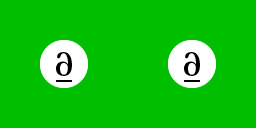
\includegraphics[width=6cm]{../images/ball_6.png}
  \caption{ball\_6.png}
  \label{fig:ball_6}
\end{figure}

\begin{figure}[H]
  \centering
  
\includegraphics[width=6cm]{../images/ball_7.png}
  \caption{ball\_7.png}
  \label{fig:ball_7}
\end{figure}

\begin{figure}[H]
  \centering
  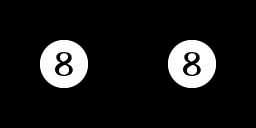
\includegraphics[width=6cm]{../images/ball_8.png}
  \caption{ball\_8.png}
  \label{fig:ball_8}
\end{figure}

\begin{figure}[H]
  \centering
  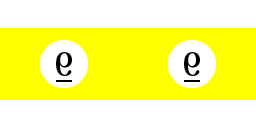
\includegraphics[width=6cm]{../images/ball_9.png}
  \caption{ball\_9.png}
  \label{fig:ball_9}
\end{figure}

\begin{figure}[H]
  \centering
  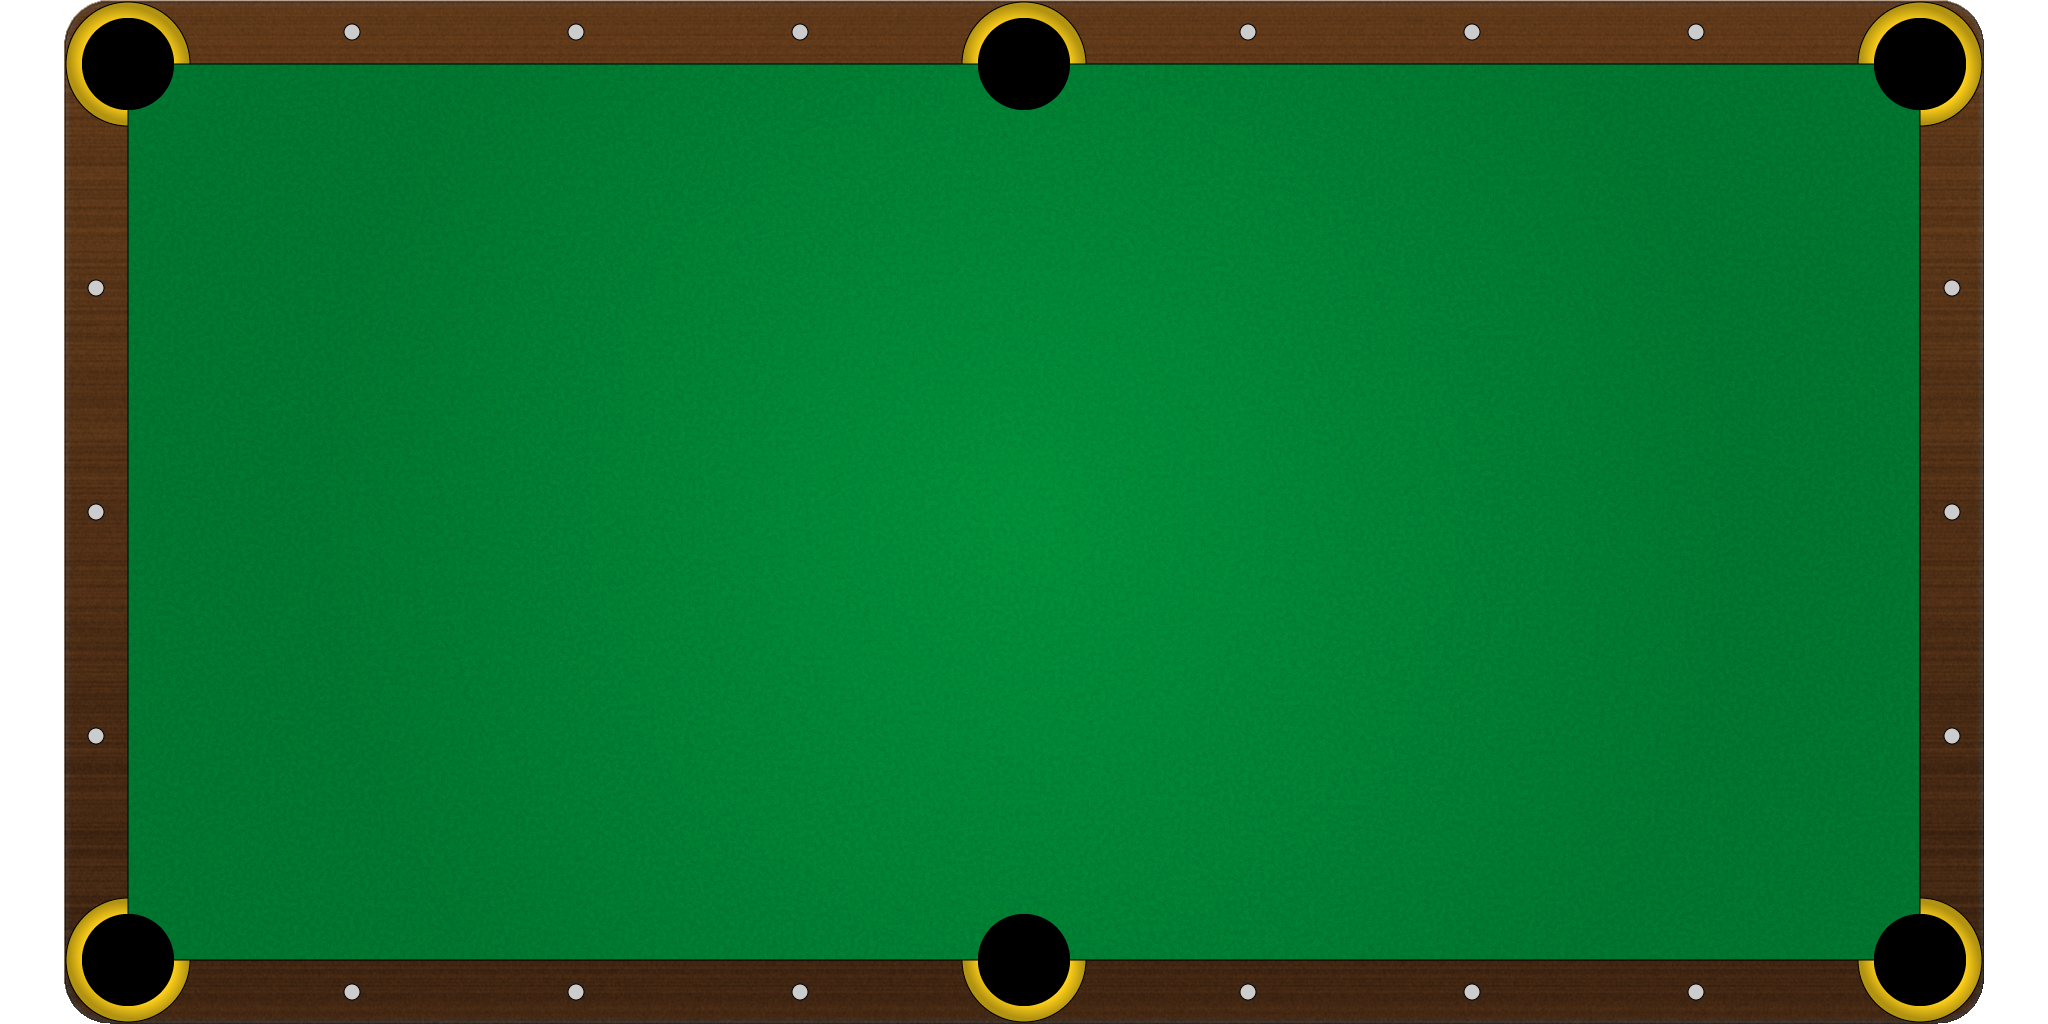
\includegraphics[width=12cm]{../images/table.png}
  \caption{table.png}
  \label{fig:table}
\end{figure}

\begin{figure}[H]
  \centering
  
\includegraphics[width=8cm]{../images/cue.png}
  \caption{cue.png}
  \label{fig:cue}
\end{figure}

\begin{figure}[H]
  \centering
  
\includegraphics[width=4cm]{../images/invalid.png}
  \caption{invalid.png}
  \label{fig:invalid}
\end{figure}

\begin{figure}[H]
  \centering
  
\includegraphics[width=8cm]{../images/turn_0.png}
  \caption{turn\_0.png}
  \label{fig:turn_0}
\end{figure}

\begin{figure}[H]
  \centering
  
\includegraphics[width=8cm]{../images/turn_1.png}
  \caption{turn\_1.png}
  \label{fig:turn_1}
\end{figure}

\begin{figure}[H]
  \centering
  
\includegraphics[width=8cm]{../images/turn_2.png}
  \caption{turn\_2.png}
  \label{fig:turn_2}
\end{figure}

\begin{figure}[H]
  \centering
  
\includegraphics[width=8cm]{../images/turn_3.png}
  \caption{turn\_3.png}
  \label{fig:turn_3}
\end{figure}

\begin{figure}[H]
  \centering
  
\includegraphics[width=8cm]{../images/win_0.png}
  \caption{win\_0.png}
  \label{fig:win_0}
\end{figure}

\begin{figure}[H]
  \centering
  
\includegraphics[width=8cm]{../images/win_1.png}
  \caption{win\_1.png}
  \label{fig:win_1}
\end{figure}

\begin{figure}[H]
  \centering
  
\includegraphics[width=8cm]{../images/win_2.png}
  \caption{win\_2.png}
  \label{fig:win_2}
\end{figure}

\begin{figure}[H]
  \centering
  
\includegraphics[width=8cm]{../images/win_3.png}
  \caption{win\_3.png}
  \label{fig:win_3}
\end{figure}

\begin{figure}[H]
  \centering
  
\includegraphics[width=12cm]{../images/title.png}
  \caption{title.png}
  \label{fig:title}
\end{figure}

\begin{figure}[H]
  \centering
  
\includegraphics[width=8cm]{../images/vshuman_0.png}
  \caption{vshuman\_0.png}
  \label{fig:vshuman_0}
\end{figure}

\begin{figure}[H]
  \centering
  
\includegraphics[width=8cm]{../images/vshuman_1.png}
  \caption{vshuman\_1.png}
  \label{fig:vshuman_1}
\end{figure}

\begin{figure}[H]
  \centering
  
\includegraphics[width=8cm]{../images/vscpu_0.png}
  \caption{vscpu\_0.png}
  \label{fig:vscpu_0}
\end{figure}

\begin{figure}[H]
  \centering
  
\includegraphics[width=8cm]{../images/vscpu_1.png}
  \caption{vscpu\_1.png}
  \label{fig:vscpu_1}
\end{figure}

\begin{figure}[H]
  \centering
  
\includegraphics[width=4cm]{../icon/icon-48.png}
  \caption{icon.ico}
  \label{fig:icon}
\end{figure}


\section{ビルド方法}
GLUTとglpngが導入されているCygwin上で、次のコマンドを入力することでビルド、実行することができる。

\begin{lstlisting}[style=text]
$ make
$ ./j16426.exe
\end{lstlisting}


\section{実行結果}
本プログラムを実行したときに表示される画面を図\ref{fig:res1}に示す。
この画面で人 vs 人か、人 vs コンピュータを選ぶと、図\ref{fig:res2}のようなゲーム画面になる。
図\ref{fig:res2}を見ると、ビリヤード台の上に3Dの球が表示されており、回転運動もしていることが分かる。

\begin{figure}[H]
  \centering
  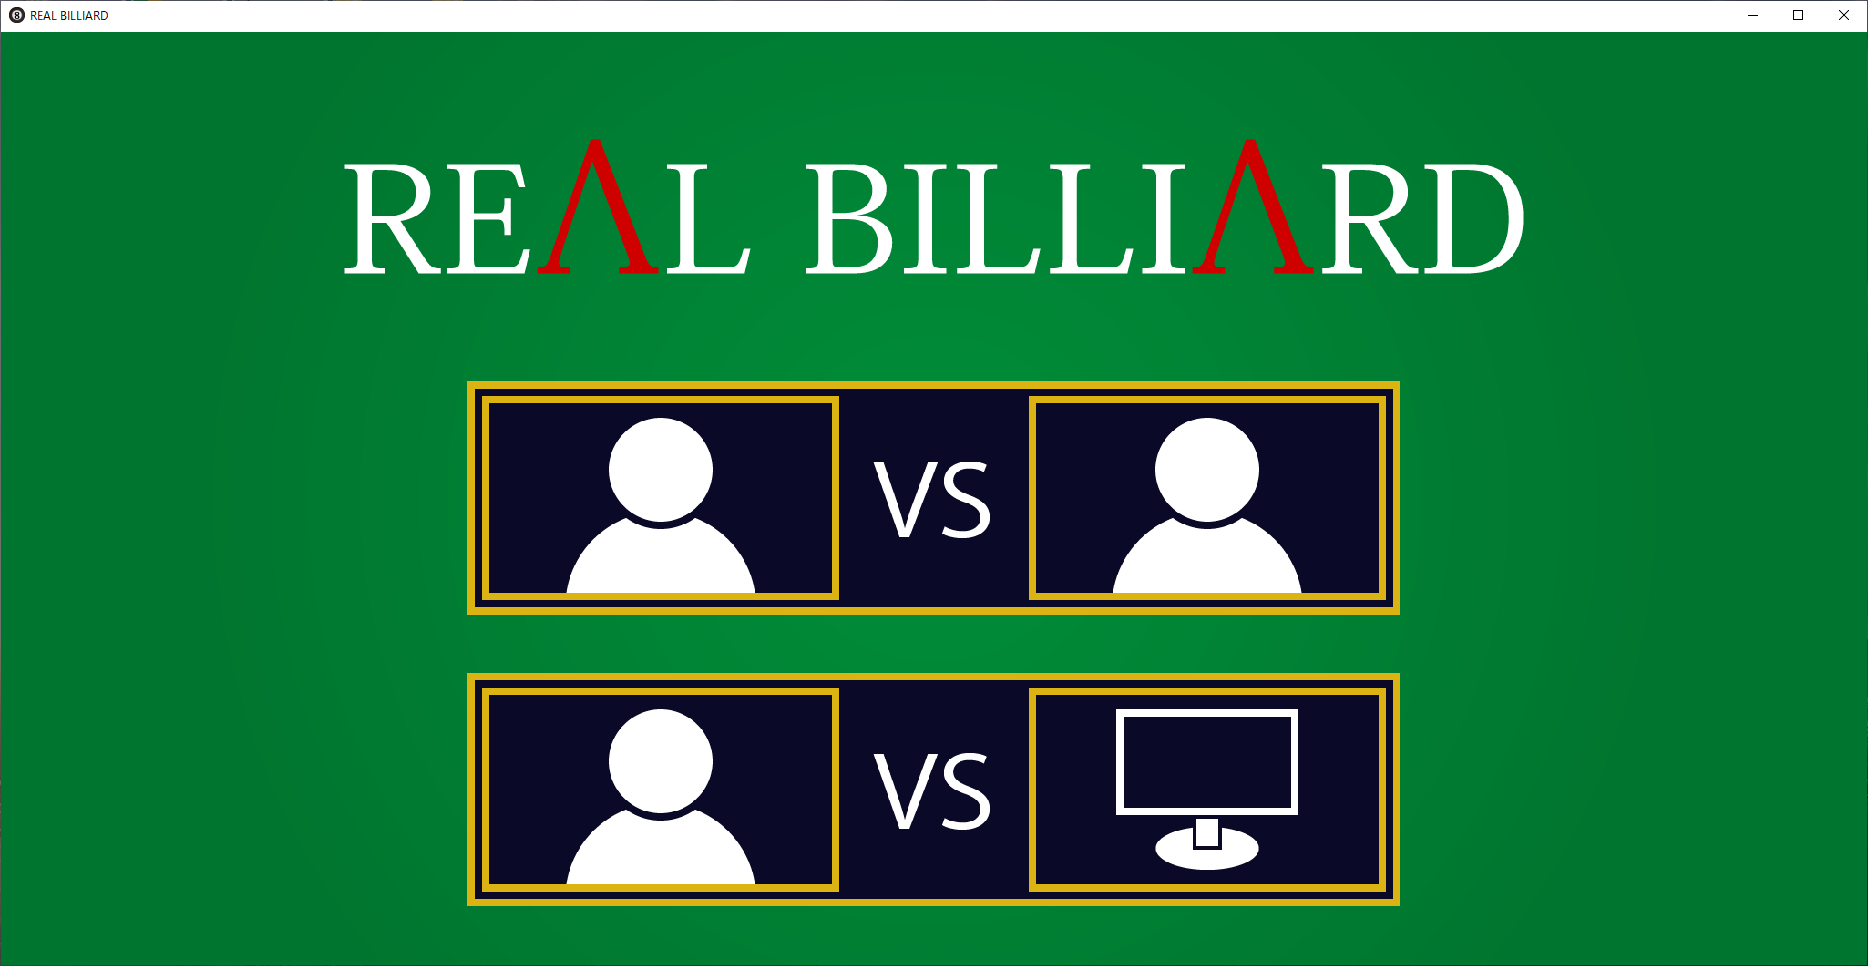
\includegraphics[width=12cm]{result1.png}
  \caption{タイトル画面}
  \label{fig:res1}
\end{figure}

\begin{figure}[H]
  \centering
  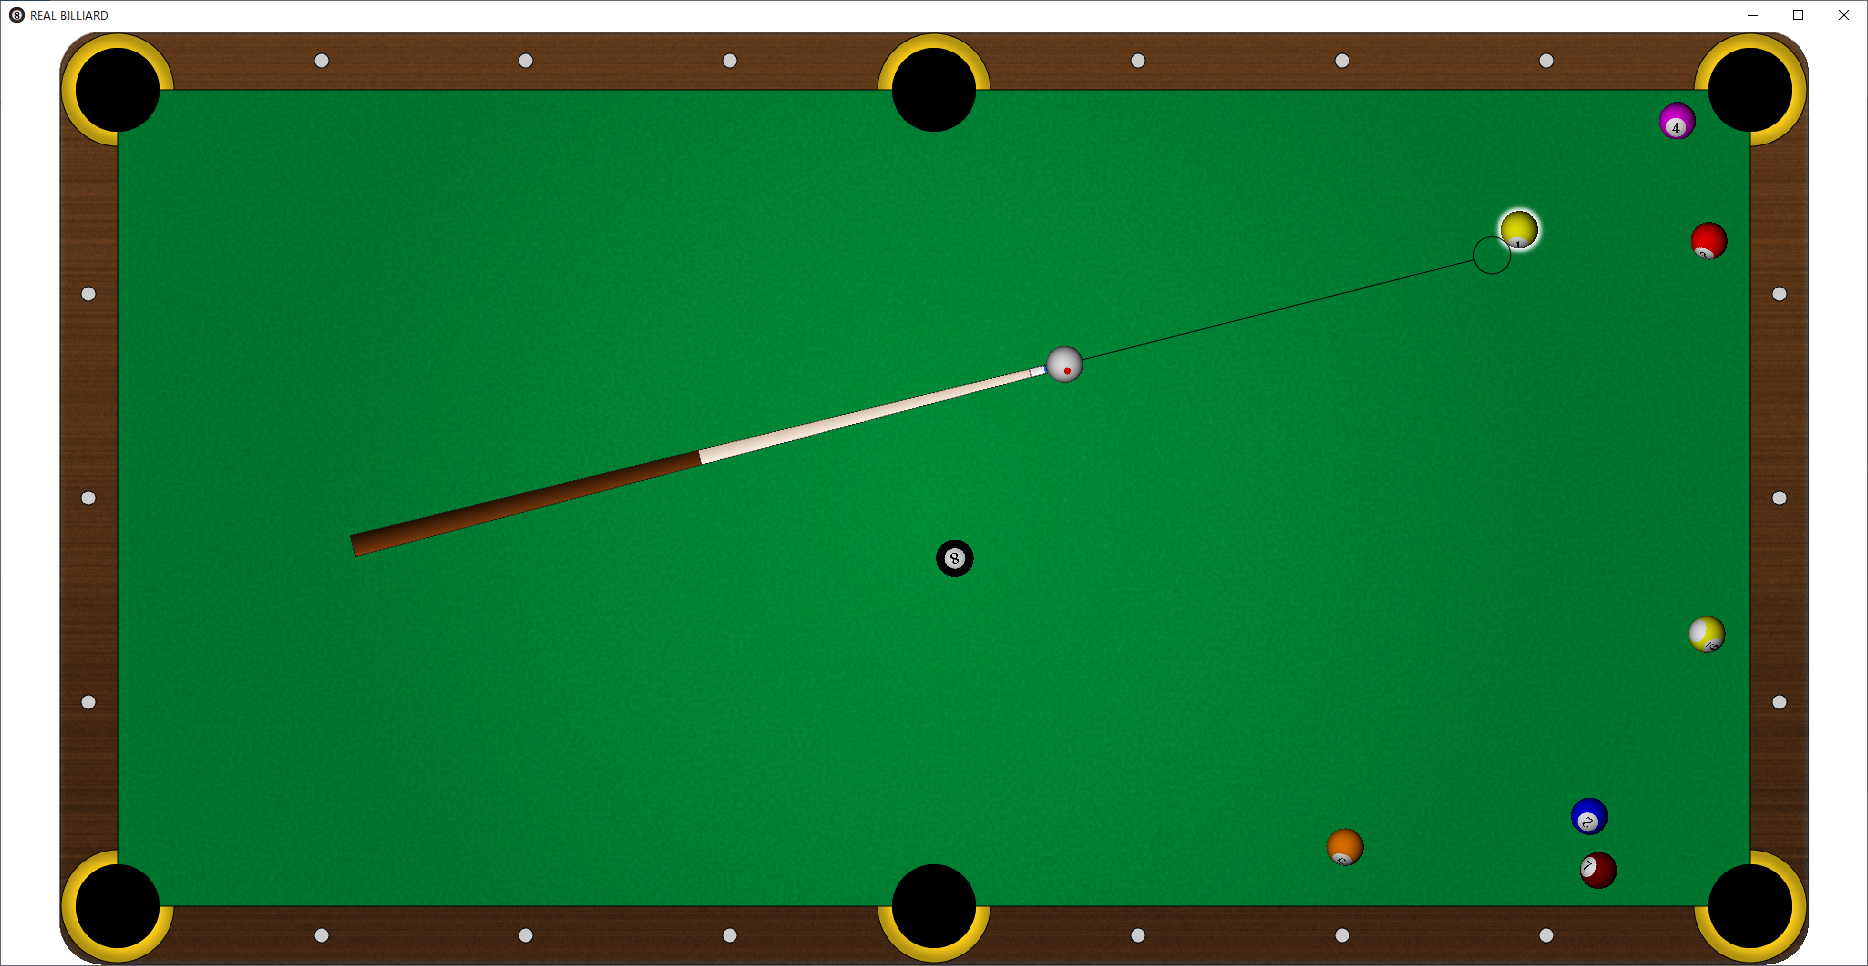
\includegraphics[width=12cm]{result2.png}
  \caption{ゲーム画面}
  \label{fig:res2}
\end{figure}

\subsection{アニメーション}
アニメーションは、\texttt{glutTimerFunc}関数を用いて、短い間隔で描画関数を呼び出すことによって実現している。
タイマーのコールバック関数である\texttt{Timer}の中でさらにタイマーを登録することで、連続的なアニメーションを表現することが出来る。

\subsection{座標系}
ウィンドウを横長になるように広げた状態を図\ref{fig:res2}, 縦長になるように縮めた状態を図\ref{fig:res3}に示す。
図\ref{fig:res2}を見ると、ウィンドウサイズに合わせて画面が拡大され、ウィンドウの中心に表示されている。
図\ref{fig:res3}を見ると、ウィンドウサイズを小さくしても見切れることなく、ウィンドウの横幅いっぱいに表示されていることが分かる。

\begin{figure}[H]
  \centering
  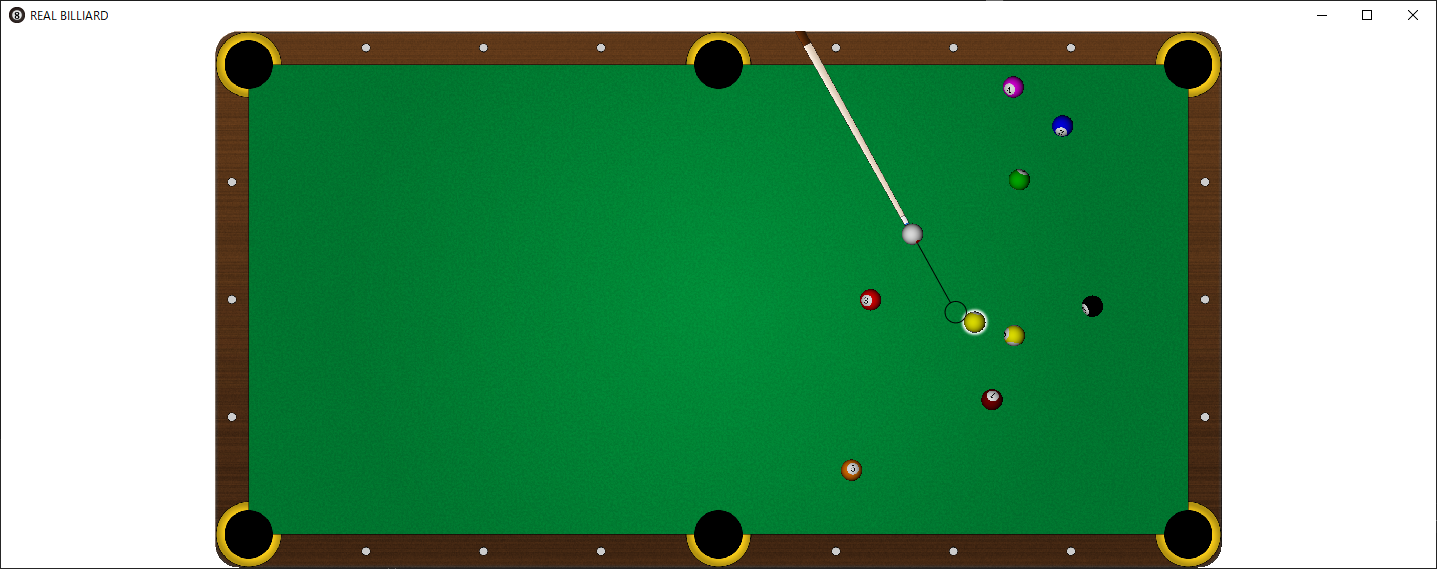
\includegraphics[width=12cm]{result3.png}
  \caption{横に長いウィンドウ}
  \label{fig:res3}
\end{figure}

\begin{figure}[H]
  \centering
  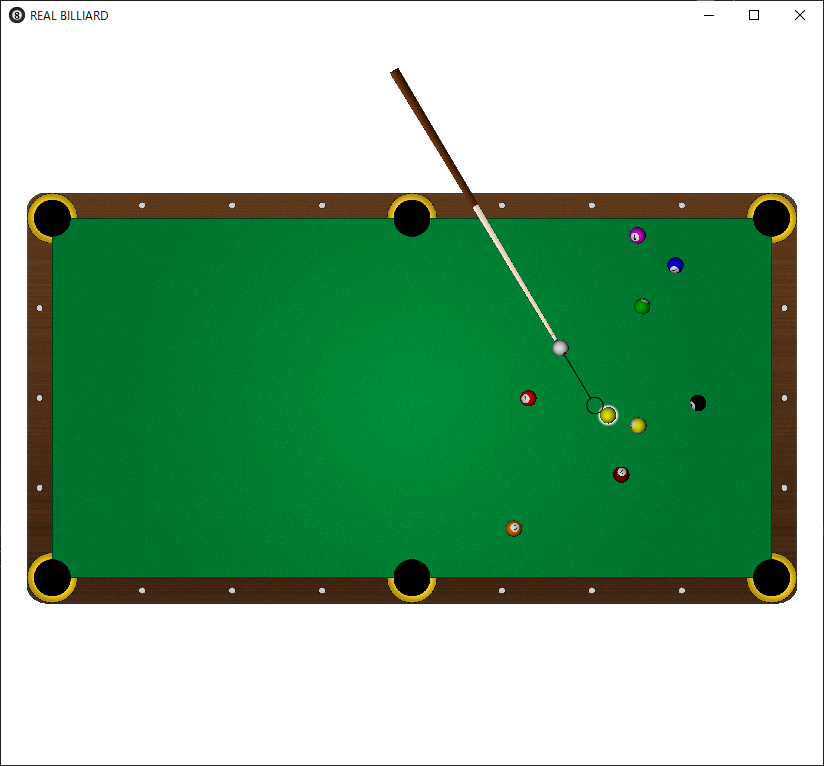
\includegraphics[width=8cm]{result4.png}
  \caption{縦に長いウィンドウ}
  \label{fig:res4}
\end{figure}

これは、ウィンドウサイズが変更された際に逐次座標系を変更しているためである。
ウィンドウが横に長い際の座標系は図\ref{fig:frame1}, 縦に長い際は図\ref{fig:frame2}のようになる。

\begin{figure}[H]
  \centering
  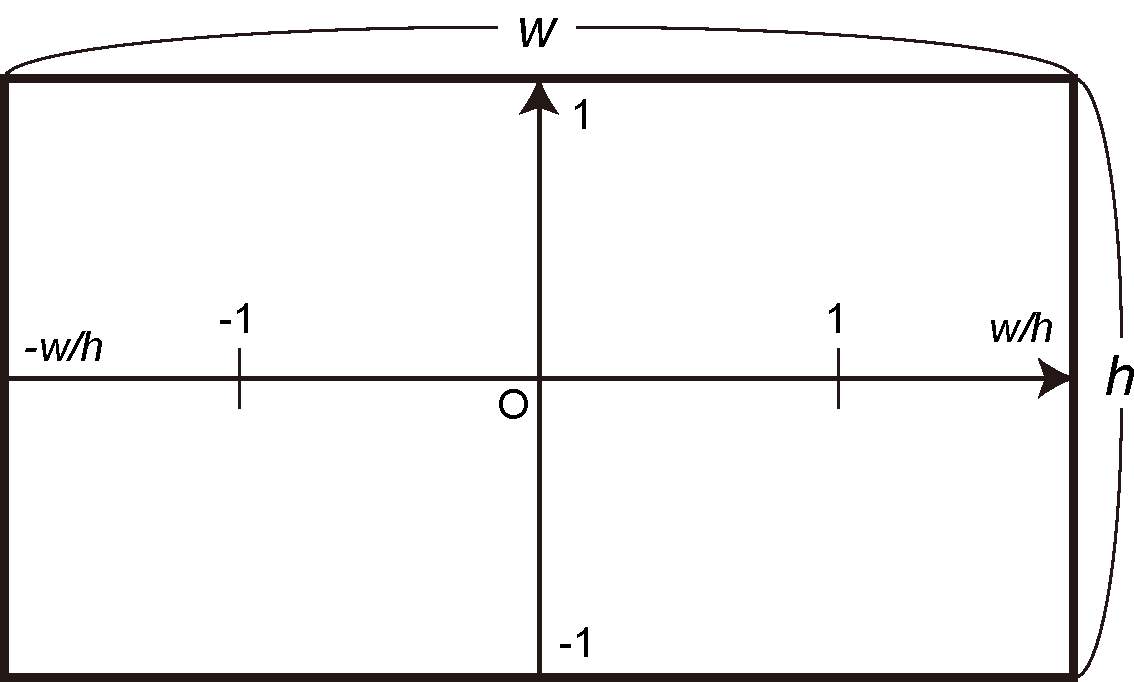
\includegraphics[width=8cm]{座標系1.pdf}
  \caption{横に長い座標系}
  \label{fig:frame1}
\end{figure}

\begin{figure}[H]
  \centering
  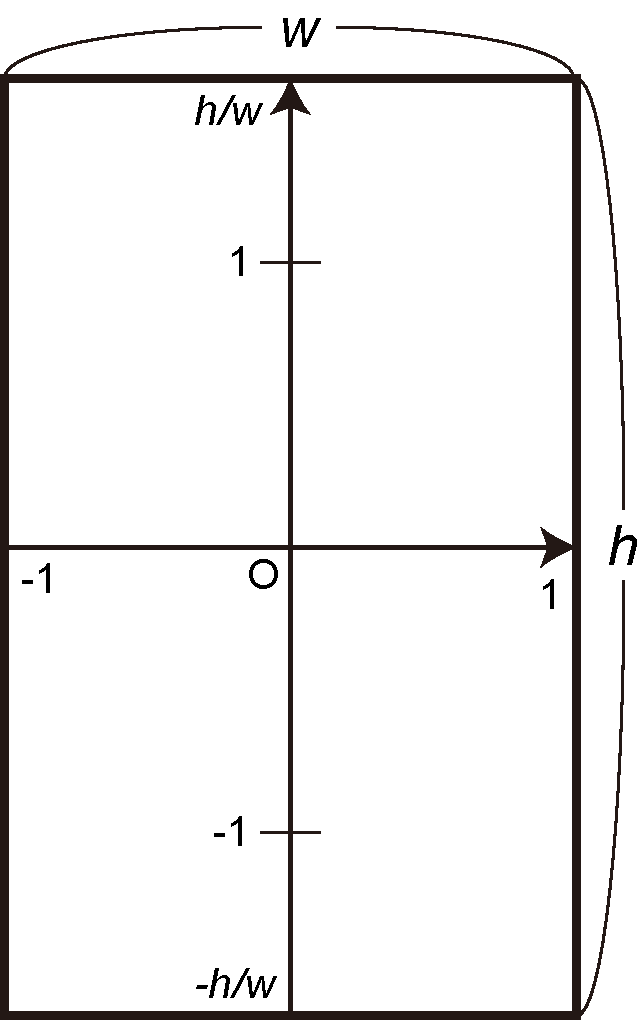
\includegraphics[width=5cm]{座標系2.pdf}
  \caption{縦に長い座標系}
  \label{fig:frame2}
\end{figure}

この設定を行っているのが\texttt{Reshape}関数である。ウィンドウサイズが変更された際に呼び出されるコールバック関数として\texttt{glutReshapeFunc}関数で登録されている。
\texttt{gluOrtho2D}という関数で画面端に対する座標を指定することができる。
これを図\ref{fig:frame1}, \ref{fig:frame2}のように設定することで、画面サイズに対する比で座標を指定することになるので、
ウィンドウサイズが変更されてもそれに合わせて拡大縮小されるようになる。
また、$x$軸方向と$y$軸方向の座標の比を1:1になるようにしているため、横長、縦長にしても画面が潰れることがない。

\subsection{球の衝突}
球の衝突処理は、ball.cの\texttt{reflectBall}関数で行っている。
図\ref{fig:parts}のように質量の等しい2つの球$a$, $b$が速度$\bvec{v_a}$, $\bvec{v_b}$で衝突した際、衝突後の速度$\bvec{v_a'}$, $\bvec{v_b'}$は式(\ref{eq:va}), (\ref{eq:vb})のようになる \cite{bib:2}。
なお、$\bvec{x_{ab}} = \bvec{x_a} - \bvec{x_b}$, $\widehat{\bvec{x}} = \dfrac{\bvec{x}}{| \bvec{x} |}$を表す。

\begin{figure}[H]
  \centering
  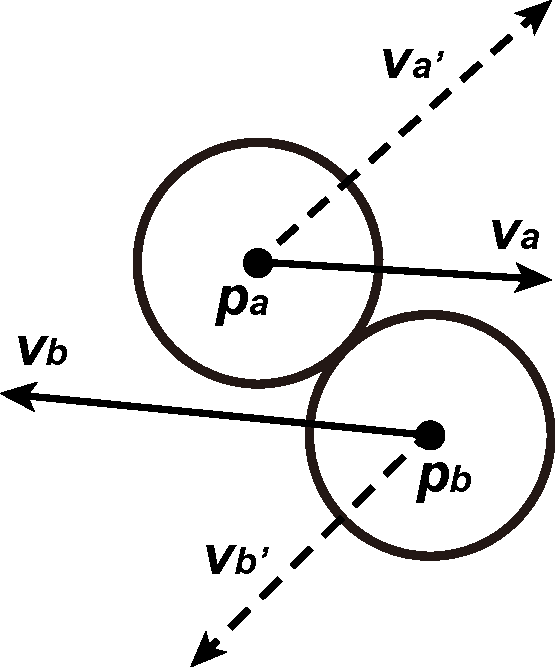
\includegraphics[width=5cm]{球の衝突.pdf}
  \caption{球の衝突}
  \label{fig:parts}
\end{figure}

\begin{equation}
  \bvec{v_a'} = \bvec{v_a} + \left( \bvec{v_{ab}} \cdot \widehat{\bvec{p_{ab}}} \right) \widehat{\bvec{p_{ab}}}
  \label{eq:va}
\end{equation}

\begin{equation}
  \bvec{v_b'} = \bvec{v_b} - \left( \bvec{v_{ab}} \cdot \widehat{\bvec{p_{ab}}} \right) \widehat{\bvec{p_{ab}}}
  \label{eq:vb}
\end{equation}

\subsection{ベクトル}
物理演算を行う際、ベクトルの計算が非常に多くなるため、vector.cにベクトルを表す構造体を定義した。
四則演算だけでなく、2つのベクトルの成す角や内積を計算する関数を作成した。
これにより、数値計算を効率的に行うことができた。

\subsection{予測線}
図\ref{fig:res2}を見ると、手球の通る軌道に線が描画されている。
これには、図\ref{fig:pre}のように、速度$\bvec{v_a}$で移動する球$a$が、静止している球$b$に衝突するかどうかを考える。

\begin{figure}[H]
  \centering
  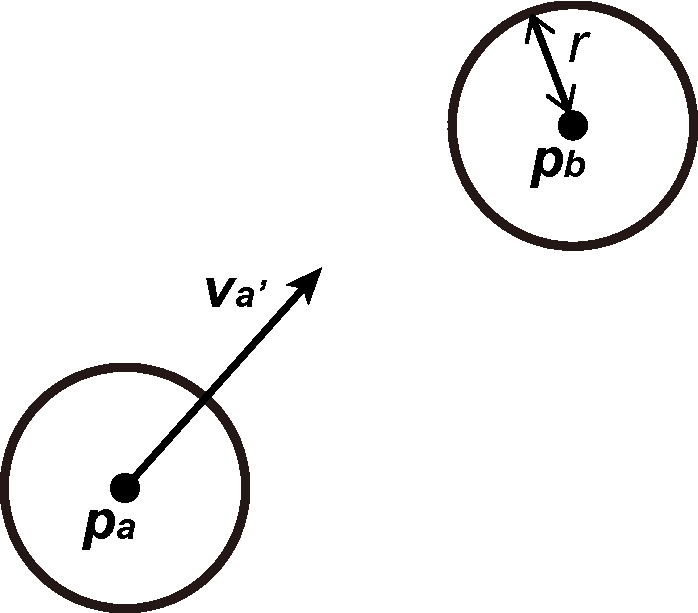
\includegraphics[width=5cm]{predict.pdf}
  \caption{ボールの衝突予想}
  \label{fig:pre}
\end{figure}

これは、点$\bvec{p_a}$を通り、傾きが$\bvec{v_a}$の直線と、点$\bvec{p_b}$の距離が$2r$以下であれば衝突する。
点$A(x_0, y_0)$と直線$ax + by + c = 0$の距離$d$は、式(\ref{eq:kyori})で与えられるため、事前に手球と衝突するかどうかを予測することができる。

\begin{equation}
  d = \frac{| ax_0 + by_0 + c |}{\sqrt{a^2 + b^2}}
  \label{eq:kyori}
\end{equation}

\subsection{コンピュータ}
図\ref{fig:com}のように、球$a$を$b$に当て、座標$p_p$に位置するポケットに落としたい場合を考える。

\begin{figure}[H]
  \centering
  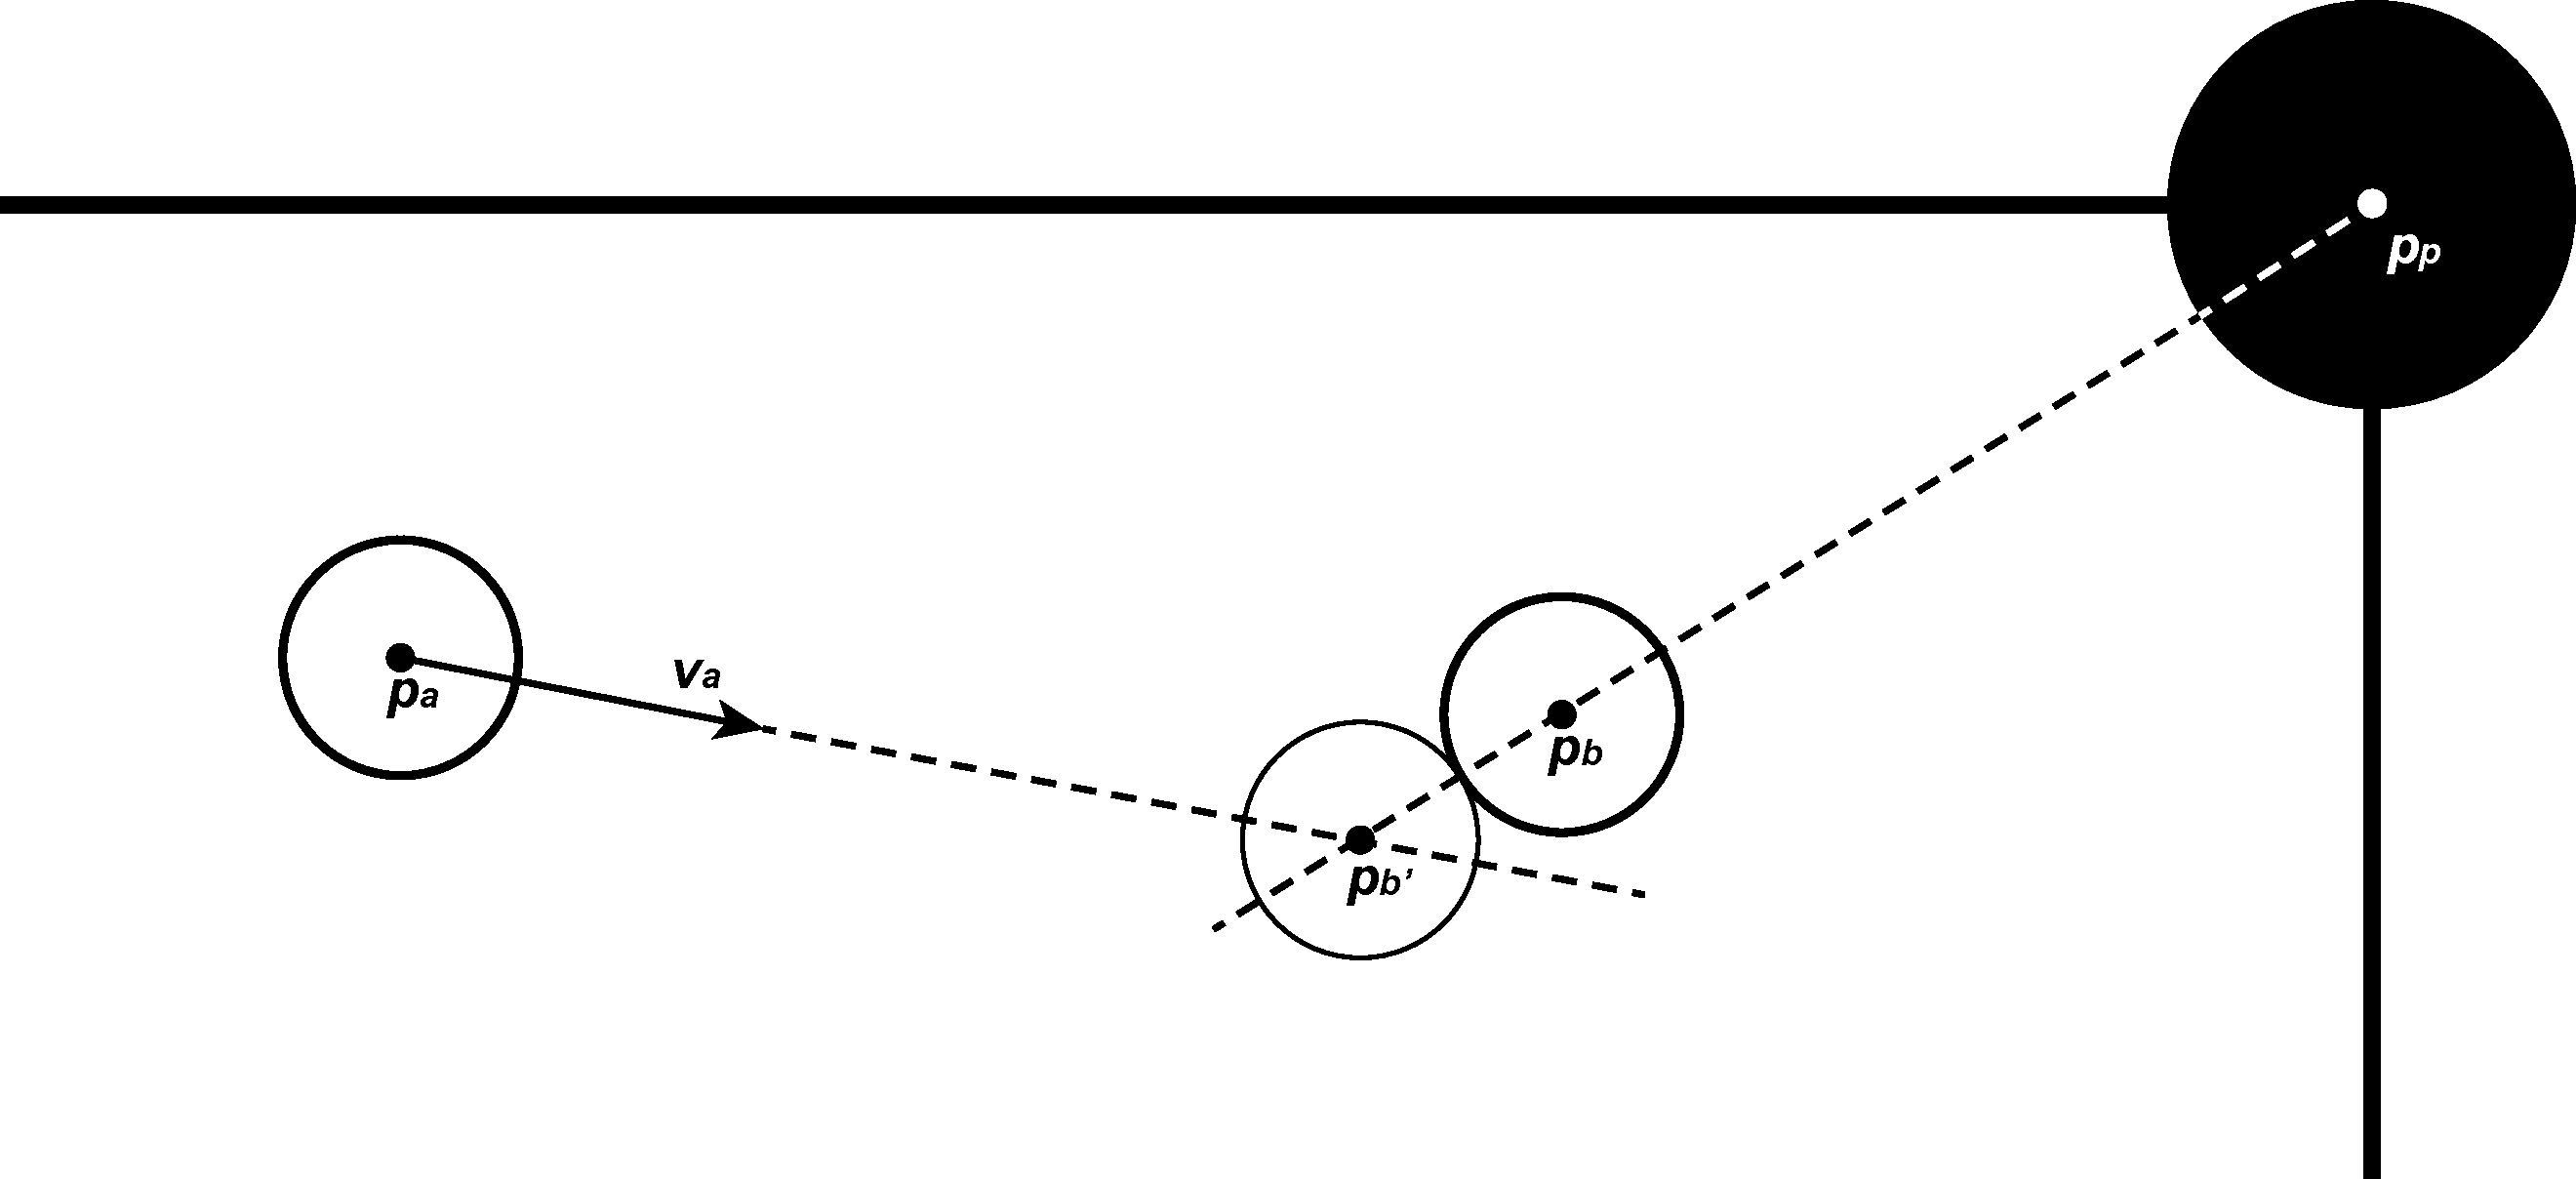
\includegraphics[width=14cm]{コンピュータ.pdf}
  \caption{コンピュータの思考}
  \label{fig:com}
\end{figure}

$p_b$と$p_p$を結ぶ線上にあり、球$b$と接する球の座標を$p_b'$とする。
このとき、球$a$を$p_b'$の方向に発射することで、球$b$をポケットに落とすことができる。

ただし、ゲーム性を考えて、本プログラムのコンピュータは毎回完璧なショットを打たず、ランダムで照準をずらすように設定してある。

\subsection{ボールの3D表示}
ボールの表示は、ball.cの\texttt{drawBall}関数で行っている。
\texttt{glTranslated}関数と\texttt{glRotated}関数で座標系を設定した後、
\texttt{gluSphere}関数で球を描画している。
このとき、\texttt{glBindTexture}関数により、テクスチャをマッピングしている。

\subsection{makeについて}
makeとは、ビルド作業を自動化するプログラムである。
Makefile内にファイルの依存関係などビルドのルールを記述しておくことで、\texttt{make}コマンドを実行するだけでビルドすることができる。
今回は、ソースファイルの変更に加え、アイコンの画像ファイルとリソースファイルが書き換えられた際も再ビルドが行われるように依存関係を記述した。


\section{感想}
OpenGLのライブラリであるGLUTを用いて、ビリヤードのプログラムを作成した。
図形を描画する処理や、ベクトルの計算を行う処理を汎用的な関数にまとめることで、完結にコードを記述できた。

今回のプログラムで一番苦戦したのは、物理演算の処理だった。
台と球の摩擦、球同士の衝突、球の回転など、考えることが山ほどあり、恐らくプログラムよりも物理で悩んでいる時間のほうが多かった。
1から物理演算を実装するのは大変だったが、摩擦係数や衝突時の速度のロスなどのパラメータを細かく設定することで、リアルな挙動が実装できた。

また、球の3D描画にも挑戦した。
2Dから3Dになるだけで、視点や光源、陰影など考慮すべき要素が増えた。
授業では扱っていない内容だったため、手探りで実装したが、球を3Dで描画することで格段にリッチな表現を実現することができた。


\section{謝辞}
物理演算を実装するにあたって、物理教員の柳沼先生にアドバイスや文献探しのお手伝いをしていただきました。
私の物理の知識だけではこのプログラムを完成させることはできなかったと思います。
柳沼先生には大変感謝しております。


\begin{thebibliography}{9}
  \bibitem{bib:1} 伊藤祥一, ``Springs of C 楽しく身につくプログラミング'', 森北出版株式会社, 2017, pp. 109--110.
  \bibitem{bib:2} ``ボール同士の衝突の公式'', 物理学の見つけ方, \texttt{\url{https://physics-htfi.github.io/classical_mechanics/005.html}}, 参照2020/2/3.
\end{thebibliography}


\end{document}
